\subsubsection{Semiconductor Devices and Transistor Circuit Analysis}

\begin{CheatsheetEntryFrame}

    \CheatsheetEntryTitle{Bipolar Junction Transistor (BJT)}

    \begin{MulticolsSoftSepRule}{2}
    
        \myul{NPN Type}

        \begin{minipage}[c]{0.3\columnwidth}
            \MinipageInheritDocumentFormatting
            \begin{center}
            \begin{circuitikz}
                \draw
                    (0,0)
                        node[npn, anchor=center](Q1){}
                    (Q1.B)
                        node[ocirc, label=left:B]{}
                    (Q1.E)
                        node[ocirc, label=below:E]{}
                    (Q1.C)
                        node[ocirc, label=above:C]{}
                ;
            \end{circuitikz}
            \end{center}
        \end{minipage}%
        \begin{minipage}[c]{0.7\columnwidth}
            \MinipageInheritDocumentFormatting
            \phantom{\small .} % TODO: Why does this work?
            \begin{center}
            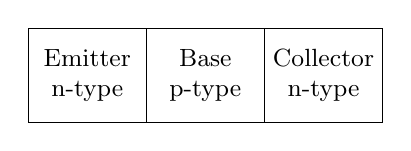
\begin{tikzpicture}
                \draw
                    (0,0)
                        rectangle ++(1.5,1.2)
                            node[pos=0.5, align=center, font={\small}]{Emitter \\ n-type}
                        rectangle ++(1.5,-1.2)
                            node[pos=0.5, align=center, font={\small}]{Base \\ p-type}
                        rectangle ++(1.5,1.2)
                            node[pos=0.5, align=center, font={\small}]{Collector \\ n-type}
                ;
            \end{tikzpicture}
            \vspace*{3mm}

            \end{center}
        \end{minipage}%
        \bigskip

        \begin{center}
            {\footnotesize\myul{\textbf{Hybrid-$\pi$ Small Signal Model}}}

            \begin{circuitikz}
                \draw
                    (0,0)
                            node[ocirc, label=left:B]{}
                        -- ++(1,0)
                            coordinate(B1)
                        to[C, l_=$C_\pi$] ++(0,-2)
                        -- ++(3.2,0)
                            coordinate(E)
                        -- ++(2.2,0)
                        to[R, l_=$r_o$] ++(0,2)
                            coordinate(C)
                        -- ++(1,0)
                            node[ocirc, label=right:C]{}
                    (B1)
                        -- ++(1.2,0)
                            coordinate(B2)
                        to[R, l_=$r_\pi$, v^>=$v_{BE}$] ++(0,-2)
                    (B2)
                        to[C, l=$C_\mu$] (E |- C)
                        %to[american controlled current source, l=$g_m v_{BE}$] (E)
                        to[american controlled current source, l=$
                                \begin{gathered}
                                    g_m v_{BE} \\
                                    \textbf{\small (or)} \\
                                    \beta i_B
                                \end{gathered}
                            $] (E)
                    (E |- C)
                        -- (C)
                    (E)
                        -- ++(0,-1)
                            node[ocirc, label=right:E]{}

                    (B1)
                        ++(-0.5,0)
                            node[currarrow, label=above:$i_B$]{}
                    (C)
                        ++(0.5,0)
                            node[currarrow, label=above:$i_C$, rotate=180]{}
                    (E)
                        ++(0,-0.5)
                            node[currarrow, label=left:$i_E$, rotate=-90]{}
                ;
            \end{circuitikz}
        \end{center}

        \emph{Forward active mode} characteristics:
        \begin{gather*}
            \begin{gathered}
                I_C = \beta I_B
                \\
                I_E = \parens{\beta + 1} I_B
            \end{gathered}
            \qquad\quad
            \beta = \frac{\alpha}{1 - \alpha}
            \qquad\quad
            I_C = \alpha I_E
        \end{gather*}
        \begin{gather*}
            I_E = I_S \parens{e^{\brackets{V_{BE} \mathbin{/} V_T}} - 1}
        \end{gather*}

        Small signal parameters:
        \begin{gather*}
            g_m = \frac{\abs*{I_C}}{V_T}
            \qquad\quad
            r_\pi = \frac{\beta}{g_m}
            \qquad\quad
            r_o = \frac{V_{CE} + V_A}{I_C}
        \end{gather*}

        Transition frequency:
        \begin{gather*}
            f_T = \frac{g_m}{2 \pi \parens{C_\pi + C_\mu}}
        \end{gather*}

        \MulticolsBreak

        \myul{PNP Type}

        \begin{center}
        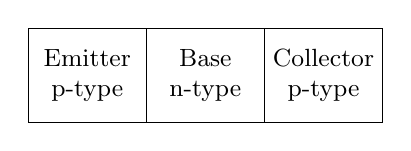
\begin{tikzpicture}
            \draw
                (0,0)
                    rectangle ++(1.5,1.2)
                        node[pos=0.5, align=center, font={\small}]{Emitter \\ p-type}
                    rectangle ++(1.5,-1.2)
                        node[pos=0.5, align=center, font={\small}]{Base \\ n-type}
                    rectangle ++(1.5,1.2)
                        node[pos=0.5, align=center, font={\small}]{Collector \\ p-type}
            ;
        \end{tikzpicture}

        \begin{circuitikz}
            \draw
                (0,0)
                    node[pnp, anchor=center, yscale=-1](Q2){}
                (Q2.B)
                    node[ocirc, label=left:B]{}
                (Q2.E)
                    node[ocirc, label=below:E]{}
                (Q2.C)
                    node[ocirc, label=above:C]{}
            ;
        \end{circuitikz}
        \end{center}

        \Todo{I don't need to know PNP transistors yet, but I should make notes on it when I have time.}

        \Todo{Also, we should maybe derive the hybrid-$\pi$ model and show the unsimplified version in the extras section?}

        \Todo{Also, I'm not 100\% sure how to organize the equations...}

        \MulticolsCleanEnd
    \end{MulticolsSoftSepRule}
    \MulticolsReduceVspaceAfter

    Basic modes:
    \begin{itemize}
        \item \emph{Forward Active} (BE forward-biased, BC reverse-biased)
        \item \emph{Reverse Active} (BE reverse-biased, BC forward-biased)
        \item \emph{Saturation} (both junctions forward-biased)
        \item \emph{Cut-off} (both junctions reverse-biased)
    \end{itemize}

\end{CheatsheetEntryFrame}

\newpage

\begin{CheatsheetEntryFrame}

    \CheatsheetEntryTitle{MOSFET}

    \begin{MulticolsSoftSepRule}{2}
        \myul{N-Channel Type}

        \begin{center}
        \begin{circuitikz}
            \draw
                (0,0)
                    node[nmos, anchor=center](Q1){}
                (Q1.G)
                    node[ocirc, label=left:G]{}
                (Q1.S)
                    node[ocirc, label=below:S]{}
                (Q1.D)
                    node[ocirc, label=above:D]{}
            ;
        \end{circuitikz}
        \end{center}
        \bigskip

        \begin{center}
            {\footnotesize\myul{\textbf{Small Signal Model}}}

            \begin{circuitikz}
                \draw
                    (0,0)
                            node[ocirc, label=above:G]{}
                        -- ++(1,0)
                            coordinate(G)
                        to[C, l_=$C_{GS}$, v^>=$V_{GS}$] ++(0,-2)
                        -- ++(2.2,0)
                            coordinate(S)
                        -- ++(2.2,0)
                        to[R, l_=$r_o$] ++(0,2)
                            coordinate(D)
                        -- ++(1,0)
                            node[ocirc, label=above:D]{}
                    (G)
                        to[C, l=$C_{GD}$] (S |- D)
                        to[american controlled current source, l=$g_m V_{GS}$] (S)
                    (S |- D)
                        -- (D)
                    (S)
                        -- ++(0,-1)
                            node[ocirc, label=right:S]{}
                ;
            \end{circuitikz}
        \end{center}

        \emph{Saturation region} characteristics:
        \begin{gather*}
            I_G = 0
            \\
            I_{DS} = \frac{1}{2} k_n \frac{W}{L} \parens{V_{GS} - V_t}^2
        \end{gather*}

        Small signal parameters:
        \begin{gather*}
            g_m
            = k_n \frac{W}{L} \parens{V_{GS} - V_t}
            = \sqrt{2 k_n \frac{W}{L} I_{DS}}
            \\
            r_o
            = \frac{1}{\lambda I_{DS}}
            = \frac{V_A + V_{DS}}{I_{DS}}
        \end{gather*}

        \MulticolsBreak

        \myul{P-Channel Type}

        \begin{center}
        \begin{circuitikz}
            \draw
                (0,0)
                    node[pmos, anchor=center](Q2){}
                (Q2.G)
                    node[ocirc, label=left:G]{}
                (Q2.S)
                    node[ocirc, label=above:S]{}
                (Q2.D)
                    node[ocirc, label=below:D]{}
            ;
        \end{circuitikz}
        \end{center}

        \Todo{I don't need to know PMOS transistors yet, but I should make notes on it when I have time.}

        \Todo{Also add discussion on enhancement/depletion-type MOSFETs?}

        \MulticolsCleanEnd
    \end{MulticolsSoftSepRule}
    \MulticolsReduceVspaceAfter

\end{CheatsheetEntryFrame}

\begin{CheatsheetEntryFrame}

    \CheatsheetEntryTitle{Miller Theorem}

    \Todo{This?}

\end{CheatsheetEntryFrame}

\Todo{(for the next page) Write something better than ``external capacitors" and ``intrinsic capacitors"? E.g. for mid-band analysis, do we just short $\si{\micro\farad}$ capacitors?}

\newpage

\begin{CheatsheetEntryFrame}

    \CheatsheetEntryTitle{Transistor Amplifier General Analysis Method} \CheatsheetEntrySubtitle{(for linear operation)}
    \bigskip

    \begin{center}
    \begin{tikzpicture}[node distance=2cm]
        \node (step1) [MyFlowchartProcess, align=center]
            {DC Analysis \\ \footnotesize (Finding Q-point values)} (step1);
        \node (step2) [MyFlowchartProcess, below of=step1, align=center]
            {Calculate Small Signal Parameters};
        \node (step3b) [MyFlowchartProcess, below of=step2, align=center]
            {Mid-Frequency \\ Analysis};
        \node (step3a) [MyFlowchartProcess, left of=step3b, align=center, xshift=-2cm]
            {Low-Frequency \\ Analysis};
        \node (step3c) [MyFlowchartProcess, right of=step3b, align=center, xshift=2cm]
            {High-Frequency \\ Analysis};

        \draw[MyFlowchartArrow] (step1) -- (step2);
        \draw[MyFlowchartArrow] (step2) -- (step3a);
        \draw[MyFlowchartArrow] (step2) -- (step3b);
        \draw[MyFlowchartArrow] (step2) -- (step3c);

        %% TODO: Make this work? The problem is, I need to make line breaks.
        %\node (tab) [align=center, right of=step2, xshift=4cm, yshift=1cm] {\scalebox{0.8}{%
        %    \begin{tabular}{|c|c|c|c|}
        %        \hline
        %        & DC Sources & AC Sources & Transistors \\\hline 
        %        DC Analysis & enable  & disable & unchanged \\\hline 
        %        Low-Freq    & disable & enable  & small signal model \\\hline
        %        Mid-Freq    & disable & enable  & small signal model \\\hline
        %        High-Freq   & disable & enable  & small signal model \\\hline
        %    \end{tabular}%
        %}};
    \end{tikzpicture}
    \end{center}

    \bigskip

    \newcommand{\TmpFormatYes}[1]{\textbf{\color{mygreen}#1}}
    \newcommand{\TmpFormatNo}[1]{\textbf{\color{myred}#1}}
    \newcommand{\TmpFormatAltA}[1]{\textbf{\color{myblue}#1}}
    \newcommand{\TmpFormatAltB}[1]{\textbf{\color{mypurple}#1}}
    \newcommand{\TmpFormatAltC}[1]{\textbf{\color{myorange}#1}}

    For each type of analysis, redraw the circuit as follows:
    \begin{center}
    \begin{tabular}{|c|c|c|c|c|c|}
        \cline{2-6}
        \multicolumn{1}{c|}{}
            & \thead{DC \\ Sources}
            & \thead{AC \\ Sources}
            & \thead{Transistors}
            & \thead{External/$\si{\micro\farad}$ \\ Capacitors}
            & \thead{Intrinsic \\ Capacitors} \\\hline 
        \thead{DC Analysis}
            & \TmpFormatYes{enable}
            & \TmpFormatNo{disable}
            & \TmpFormatYes{unchanged}
            & \TmpFormatAltC{open}
            & \TmpFormatAltC{open} \\\hline 
        \thead{Low-Freq}
            & \TmpFormatNo{disable}
            & \TmpFormatYes{enable}
            & \TmpFormatAltA{small signal model} %\makecell{small signal \\ model}
            & \TmpFormatYes{keep}
            & \TmpFormatAltC{open} \\\hline
        \thead{Mid-Freq}
            & \TmpFormatNo{disable}
            & \TmpFormatYes{enable}
            & \TmpFormatAltA{small signal model}
            & \TmpFormatAltB{short}
            & \TmpFormatAltC{open} \\\hline
        \thead{High-Freq}
            & \TmpFormatNo{disable}
            & \TmpFormatYes{enable}
            & \TmpFormatAltA{small signal model}
            & \TmpFormatAltB{short}
            & \TmpFormatYes{keep} \\\hline
    \end{tabular}
    \end{center}

    %{\footnotesize External capacitors are $\si{\micro\farad}$ capacitors outside of the transistors. Intrinsic capacitors are capacitances found in the transistor small signal model.}
    
    \bigskip
    \SoftHLine
    %\bigskip

    \begin{MulticolsSoftSepRule}{2}

        \myul{DC Analysis}
        \begin{enumerate}
            \item Redraw the circuit appropriately.
            \item Assume linear operation:
            \begin{itemize}
                \item BJTs are \emph{forward active} $\to$ \Todo{}
                \item MOSFETs are in \emph{saturation} $\to$ \Todo{}
            \end{itemize}
            \item Check that the linear operation assumptions are met:
            \begin{itemize}
                \item NPN BJTs require \Todo{this}
                \item N-Channel MOSFETs require $V_{GS} > V_t$
            \end{itemize}
            \item Apply circuit analysis to find:
            \begin{itemize}
                \item $I_C$ and $V_{CE}$ {\footnotesize {}[for NPN BJTs]}
                \item $I_D$ and $V_{DS}$ {\footnotesize {}[for N-Channel MOSFETs]}
            \end{itemize}
        \end{enumerate}

        \bigskip
        \SoftHLine
        \bigskip

        \myul{Mid-Frequency Analysis}

        Redraw the circuit appropriately, then apply circuit analysis techniques to find:
        \begin{itemize}
            \item gain
            \item input/output resistance
        \end{itemize}

        %\bigskip
        %\SoftHLine
        %\bigskip
        \MulticolsBreak

        \myul{Low-Frequency Analysis}

        Redraw the circuit appropriately, then apply the \linebreak \emph{short circuit time constant method} to find the \linebreak lower cut-off frequency $f_L$:
        \begin{gather*}
            f_L
            = \frac{1}{2 \pi}
            \sum_{i=1}^n \frac{1}{\tau_i}
            \qquad
            \tau_i = C_i R_{sci}
        \end{gather*}
        Calculate a $\tau_i$ for every capacitor $C_i$.

        $R_{sci}$ is the Th\'evenin resistance seen by $C_i$ \linebreak with all other capacitors \textbf{\myul{shorted}}.

        \bigskip
        \SoftHLine
        \bigskip

        \myul{High-Frequency Analysis}

        Redraw the circuit appropriately, then apply the \linebreak \emph{open circuit time constant method} to find the \linebreak upper cut-off frequency $f_H$:
        \begin{gather*}
            f_H
            = \frac{1}{
                \displaystyle
                \brackets*{
                    2 \pi \sum_{i=1}^n \tau_i
                }
            }
            \qquad
            \tau_i = C_i R_{oci}
        \end{gather*}
        Calculate a $\tau_i$ for every capacitor $C_i$.

        $R_{oci}$ is the Th\'evenin resistance seen by $C_i$ \linebreak with all other capacitors \textbf{\myul{opened}}.
        
        %\MulticolsCleanEnd % TODO: Why is this not needed?
    \end{MulticolsSoftSepRule}
\end{CheatsheetEntryFrame}

